\subsection{Host - Kubuntu 16.04 (Zeroconf)}

Die Konfiguration der IP-Adressen erfolgt �ber das Zero Configuration Networking System (Zeroconf). Dazu muss am Host-PC der Dienst Avahi (avahi-daemon) installiert sein. Dieser ist auf den meisten Linux Systemen bereits vorinstalliert.\\ 
  
Zur Konfiguration unter Linux Kubuntu 16.04 muss zuerst "`Netzwerkverbindungen"' ge�ffnet werden. 
Dazu klickt man mit der rechten Maustaste auf das Netzwerksymbol in Infobereich rechts unten. Nun kann die Option "`Netzwerkverbindungen einrichten..."' ausgew�hlt werden.

\begin{figure}[ht]
  \centering
  
\includegraphics[scale=1.0]{images/OTG_NetzwerkverbindungenIcon.png}	
  
\includegraphics[scale=0.42]{images/OTG_NetzwerkverbindungenOpen.png}	
  %	\caption{}
  \label{OTG_LINUX_NetzwerkverbindungenApp}
\end{figure}


Danach kann die neue "`Kabelnetzwerkverbindung"' umbenannt werden, z.~B. in Raspberry Pi Zero. Erkennen kann man das Netzwerk an der Mac-Adresse die man bei "`g\_ether.host\_addr"' angegeben hat (z.~B. 00:01:02:03:04:05).  


\begin{figure}[ht]
  \centering
  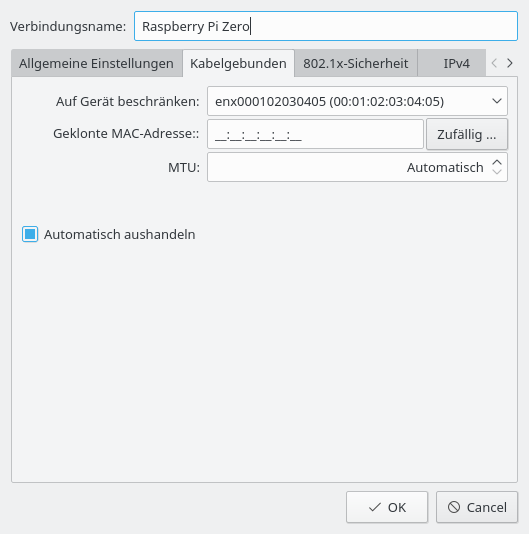
\includegraphics[scale=0.45]{images/OTG_Pi_Verbindungsname.png}
	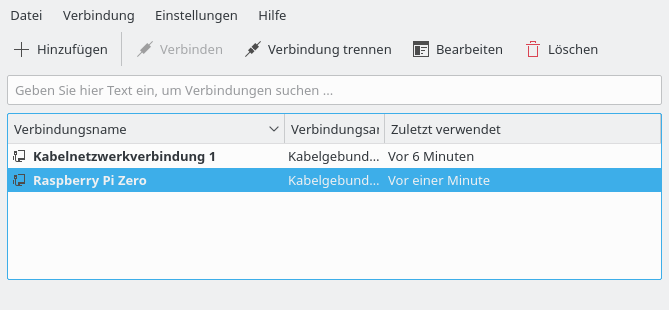
\includegraphics[scale=0.45]{images/OTG_Netzwerkverbindungen.png}
%	\caption{}
  \label{OTG_LINUX_Netzwerkverbindungen}
\end{figure}


Am Host-PC muss bei den IPv4-Einstellungen Methode "`Link-Local"' eingestellt sein.  


\begin{figure}[ht]
  \centering
  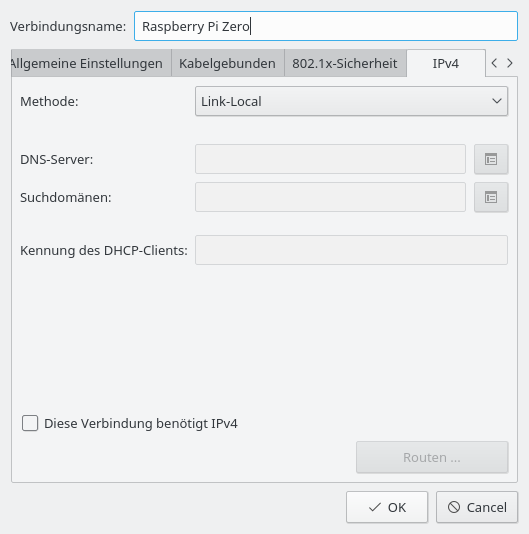
\includegraphics[scale=0.45]{images/OTG_IPv4.png}
%	\caption{}
  \label{OTG_LINUX_IPV4}
\end{figure}
